\documentclass[professionalfonts,table,aspectratio=1610]{beamer}

\usepackage[spanish]{babel}
\usepackage{iwona}
\usepackage[T1]{fontenc}
\usepackage[utf8]{inputenc}
\usepackage{amsmath,amssymb}
\usepackage{multicol,color}
\usepackage{beamerthemesplit}
\usepackage{graphicx,subfigure}
\usepackage{bm,bbm,bbding,units}
\hypersetup{colorlinks=true,allcolors=magenta}

\usepackage{texnames}
\usepackage{natbib}
\usepackage{tikz}
\usetikzlibrary{positioning}
\usetikzlibrary{arrows.meta}

\usetheme{Darmstadt}
\usecolortheme{seagull}
\setbeamercovered{transparent}
\setbeamertemplate{footline}[frame number]
\setbeamertemplate{navigation symbols}{}
\mode<handout>{
  \usepackage[bar]{beamerthemetree}
  \beamertemplatesolidbackgroundcolor{black!5}}

\renewcommand{\newblock}{}


\title{Segunda Escuela de Primavera en Teledetección}
\subtitle{Presentación}
\author[Frery-Medeiros]{Alejandro C.\ Frery\and Antonio C.\ Medeiros}
\institute[UFAL]{
\includegraphics[width=.3\linewidth]{laccan.pdf}\\
Universidade Federal de Alagoas
}
\date{Agosto de 2017}

%\logo{\includegraphics[width=.04\linewidth]{ufal.eps}}

\setbeamercovered{dynamic}
%\AtBeginSection[]{\frame{\frametitle{Resumo}\tableofcontents[current]}}

\begin{document}

\frame{\titlepage}

\begin{frame}{Agradecimientos}
Esta visita es possible gracias a los organizadores y a la IEEE GRSS.
\end{frame}

\begin{frame}{El viaje}
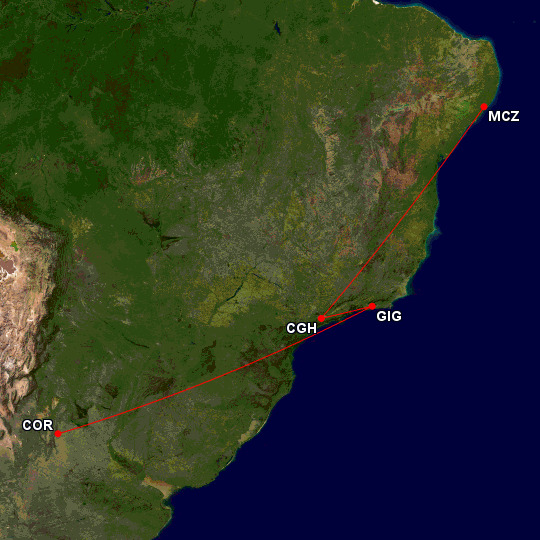
\includegraphics[width=.6\linewidth]{MCZ-CGH-GIG-COR}
\end{frame}

\begin{frame}{¿De dónde venimos? Maceió}
\includegraphics<1>[width=\linewidth]{PontaVerde}
\includegraphics<2>[width=\linewidth]{Piscinas1}
\includegraphics<3>[width=\linewidth]{Piscinas2}
\includegraphics<4>[width=\linewidth]{Barquinho}
\end{frame}

\begin{frame}
 \frametitle{Objetivos}
 Conocer y usar
\begin{itemize}
\item Propiedades estadísticas de imágenes SAR y PolSAR
\item R
\item Rmarkdown
\end{itemize}
\end{frame}

\begin{frame}{Propiedades Estadísticas}
\begin{itemize}[<+-| alert@+>]
\item Los datos SAR/PolSAR son intrínsecamente estocásticos.
\item Podemos combatir la aleatoriedad, o vivir con ella.
\item Hay mucha información útil contenida en las propiedades estadísticas.
\item Muchas de las mejores técnicas de procesamiento, análisis y asimilación de estos datos aprovechan esas propiedades.
\end{itemize}
\end{frame}

\begin{frame}{R}
Es una plataforma para hacer estadística computacional y gráficos de gran calidad que:
\begin{itemize}
\item Es \textit{FLOSS}.
\item Tiene el respaldo de una comunidad activa y colaborativa.
\item Ofrece una gran diversidad de herramientas.
\item Se caracteriza por brindar resultados de excelente calidad numérica.
\end{itemize}
\end{frame}

\begin{frame}{Rmarkdown}

\begin{itemize}
\item Lenguaje de marcación que integra \LaTeX, \BibTeX, R, C, C++ y muchos otros lenguajes.
\item Permite exportar para \LaTeX, HTML y Word (¡los dioses los perdonen!).
\item Excelentes libros se han escrito en Markdown.
\item Este es un ``libro'' interactivo: pueden editar su contenido y ver los resultados.
\end{itemize}
\end{frame}

\begin{frame}{Github}
Es una plataforma de colaboración.

El curso está disponible (y en eterna construcción) en \url{https://github.com/acfrery/SAR-PolSAR-Course}

\end{frame}

\begin{frame}{Empezando\dots}
\begin{enumerate}
\item Clonar el repositorio
\item Abrir (en RStudio) el archivo NotebookCompleto.Rmd
\item Knit -> Knit to HTML
\end{enumerate}
\end{frame}

{ % brace to limit the scope of \setbeamertemplate 
\setbeamertemplate{background canvas}{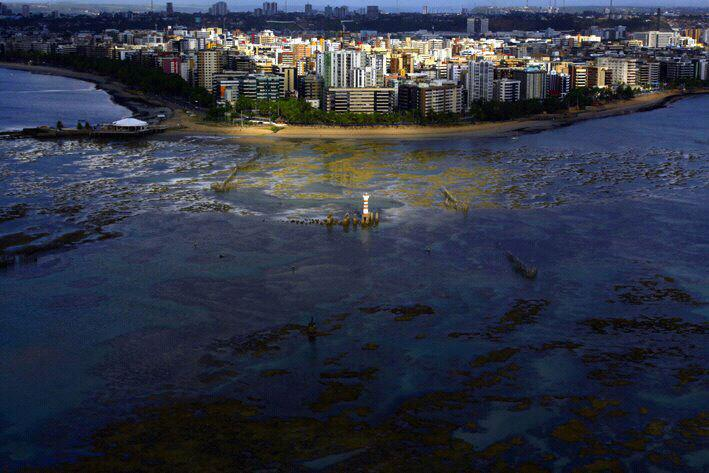
\includegraphics 
	[width=\paperwidth,height=\paperheight]{AmanhecerMaceio.jpg}} 

\begin{frame}[plain] 
\mbox{}\vskip12em
\begin{alertblock}{Contacto:}
Alejandro C. Frery\\
\texttt{acfrery@laccan.ufal.br}\\
\texttt{http://sites.google.com/site/acfrery}\\
\HandRight~\framebox{Maestría, Programas de Intercambio y Pasantías}~\HandLeft
\end{alertblock}
\end{frame} 
}

\end{document}